\documentclass{article}
\usepackage{tikz,tkz-euclide}
\usetkzobj{all}
\usetikzlibrary{arrows,calc}

\begin{document}

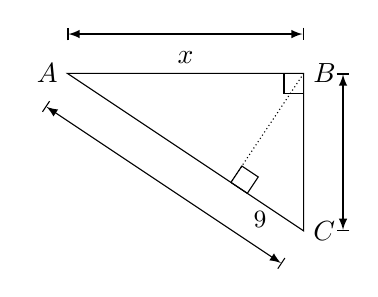
\begin{tikzpicture}
    \coordinate (A) at (0,0);
    \coordinate (B) at (3,0);
    \coordinate (C) at (3,-2);
    \coordinate (D) at ($(A)!(B)!(C)$);
    \draw (A) -- (B)
            node[pos=0,left] {$A$}
            node[midway,above] {$x$}
            node[pos=1,right] {$B$} --
          (C) -- (D)
            node[pos=0,right] {$C$}
            node[pos=0.6,below] {\small 9} -- cycle;
    \draw[densely dotted] (B) -- (D);
    \tkzMarkRightAngle (A,B,C);
    \tkzMarkRightAngle (B,D,C);
    \draw [|<->|,>=latex] ($(A)!0.5cm!-90:(C)$) -- ($(C)!0.5cm!90:(A)$);
    \draw [|<->|,>=latex] ($(B)!0.5cm!-90:(A)$) -- ($(A)!0.5cm!90:(B)$);
    \draw [|<->|,>=latex] ($(C)!0.5cm!-90:(B)$) -- ($(B)!0.5cm!90:(C)$);
\end{tikzpicture}

\end{document}